% Figure from MATH 556 notes, section 36 (added, not from lecture). Compile with the notes preamble.
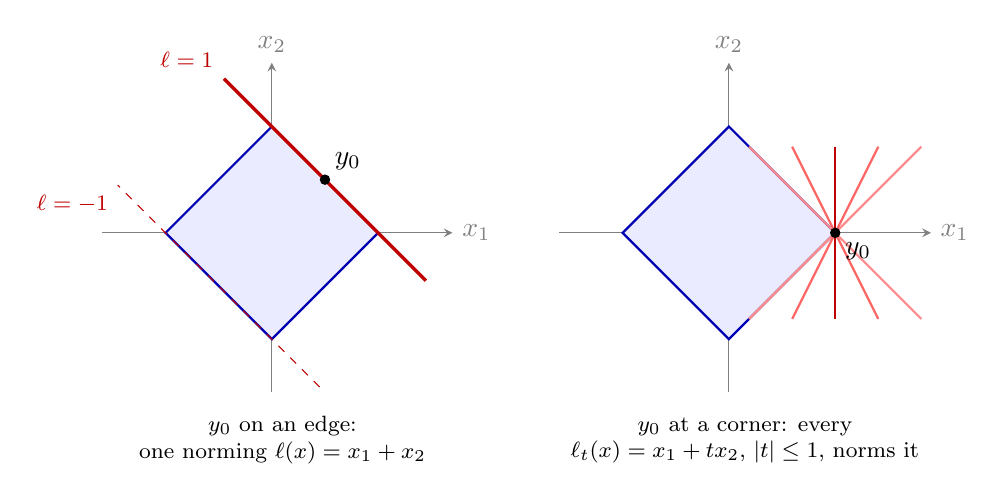
\begin{tikzpicture}[scale=1.35, >=stealth]
  \begin{scope}
    \draw[->, gray] (-1.6,0) -- (1.7,0) node[right] {$x_1$};
    \draw[->, gray] (0,-1.5) -- (0,1.6) node[above] {$x_2$};
    \fill[blue!8] (1,0) -- (0,1) -- (-1,0) -- (0,-1) -- cycle;
    \draw[thick, blue!70!black] (1,0) -- (0,1) -- (-1,0) -- (0,-1) -- cycle;
    \draw[very thick, red!75!black] (1.45,-0.45) -- (-0.45,1.45) node[above left, font=\footnotesize] {$\ell = 1$};
    \draw[dashed, red!75!black] (0.45,-1.45) -- (-1.45,0.45) node[below left, font=\footnotesize] {$\ell = -1$};
    \fill (0.5,0.5) circle (1.4pt) node[above right] {$y_0$};
    \node[font=\footnotesize, align=center] at (0.1,-1.95) {$y_0$ on an edge: \\ one norming $\ell(x) = x_1 + x_2$};
  \end{scope}
  \begin{scope}[xshift=4.3cm]
    \draw[->, gray] (-1.6,0) -- (1.9,0) node[right] {$x_1$};
    \draw[->, gray] (0,-1.5) -- (0,1.6) node[above] {$x_2$};
    \fill[blue!8] (1,0) -- (0,1) -- (-1,0) -- (0,-1) -- cycle;
    \draw[thick, blue!70!black] (1,0) -- (0,1) -- (-1,0) -- (0,-1) -- cycle;
    \foreach \t/\c in {-1/red!45, -0.5/red!60, 0/red!75!black, 0.5/red!60, 1/red!45} {
      \draw[thick, \c] ({1-1.35*\t*0.6},{1.35*0.6}) -- ({1+1.35*\t*0.6},{-1.35*0.6});
    }
    \fill (1,0) circle (1.4pt) node[below right] {$y_0$};
    \node[font=\footnotesize, align=center] at (0.15,-1.95) {$y_0$ at a corner: every \\ $\ell_t(x) = x_1 + t x_2$, $|t| \le 1$, norms it};
  \end{scope}
\end{tikzpicture}
